\documentclass[10pt]{beamer}

\usepackage{ 
    amsmath,
    amssymb,
    array,
    apacite,
    beamerthemesplit,
    bm,
    booktabs,
    catchfilebetweentags,
    color,
    colortbl,
    csquotes,
    enumitem,
    epigraph,
    fancyvrb,
    fontawesome,
    graphicx,
    hyperref,
    pifont,
    scalerel,
    tabularx,
    tikz,
    tikz-qtree,
    xcolor,
    xfrac}


% Theme modifications
\usetheme[progressbar=foot]{metropolis}
\addtobeamertemplate{frametitle}{}{\vspace{1em}}
\renewcommand{\emph}[1]{{{\color{red}#1}}}
\renewcommand\bibliographytypesize{\footnotesize}

\setbeamercolor{block title}{use=structure,fg=black,bg=black!15!white}
\setbeamercolor{block body}{use=structure,fg=black,bg=black!10!white}

\setbeamercolor{background canvas}{bg=white}
%\setbeamercolor{normal text}{fg=black}

\renewcommand\bibliographytypesize{\footnotesize}

\setlist[enumerate]{label=\bf\alph*)}

\addtobeamertemplate{block begin}{\vskip +1.5\bigskipamount}{}
\addtobeamertemplate{block end}{}{\vskip -1.5\bigskipamount}


% Super lazy shorthands
\newcommand{\e}[1]{\emph{#1}}
\newcommand{\strng}[1]{{{\color{jade}#1}}}

\newcommand{\bi}{\begin{itemize}}
\newcommand{\ei}{\end{itemize}}
\renewcommand{\i}{\item[$\bullet$]<+->}

\newcommand{\ex}[1]{\begin{block}{#1}\vspace{0pt}}
\newcommand{\xe}{\end{block}\vspace{3ex}}

\newcommand{\beq}{\begin{eqnarray*}}
\newcommand{\eeq}{\end{eqnarray*}}

\renewcommand{\c}[2]{{\color{#1}\texttt{#2}}}

\newcommand{\code}[1]{\texttt{#1}}


% Font
\usefonttheme[onlymath]{serif}

% Unusual symbols
\newcommand{\cmark}{\ding{51}}% Check mark
\newcommand{\xmark}{\ding{55}}% Cross mark
\let\lightning\faBolt % Lightning bolt


% Colors
\definecolor{amber}{rgb} {0.99, 0.75, 0.20}
\definecolor{violet}{rgb}{0.55, 0.20, 0.90}
\definecolor{jade}{rgb}  {0.00, 0.66, 0.42}
\definecolor{blue}{rgb}  {0.00, 0.39, 0.64}
\definecolor{gold}{rgb}  {1.00, 0.82, 0.00}
\definecolor{lightgrey}{rgb}  {0.85, 0.85, 0.85}
\definecolor{offwhite}{rgb}   {0.965, 0.965, 0.965}
\definecolor{paleyellow}{rgb} {1, .975, 0.85}
\definecolor{bordeaux}{rgb}   {0.50, 0.10, 0.10}
\definecolor{royalblue}{rgb}  {0.26, 0.41, 0.88}
\definecolor{darkgreen}{rgb}  {0.10, 0.50, 0.10}

\definecolor{titleCiteAColor}{rgb} {0.5, 0.7, 0.85}
\definecolor{titleCiteColor}{rgb}  {0.5, 0.7, 0.85}


% Hyperlink colors
\hypersetup{
    citecolor=,  % Clear global citecolor, see below
    colorlinks=true,
    linkcolor=blue,
    filecolor=magenta,      
    urlcolor=cyan,
}


% Extend cite for color
\let\plainCiteA\citeA
\renewcommand{\citeA}[2][gray]{{\color{#1}\plainCiteA{#2}}}
\let\plainCite\cite
\renewcommand{\cite}[2][gray]{{\color{#1}\plainCite{#2}}}

\newcommand{\titleCiteA}[1]{\citeA[titleCiteAColor]{#1}}
\newcommand{\titleCite}[1]{\cite[titleCiteColor]{#1}}


% Math and logic notation
\newcommand{\given}{{ \mid }}

\newcommand{\lxor}{\veebar}
\renewcommand{\l}[1]{\mbox{ \sc{#1} }}

\renewcommand{\therefore}{\Rightarrow}
\renewcommand{\implies}{\rightarrow}
\newcommand{\equivalent}{\leftrightarrow}
\newcommand{\nonequivalent}{\not\leftrightarrow}


% Graphics
\usepackage{graphicx}
\graphicspath{ {p/} }

\usetikzlibrary{trees}
\usetikzlibrary{tikzmark}


% Title page defaults
\author[shortname]{Joachim Vandekerckhove\\Michael D. Lee}
\date{}



\title{Multinomial Processing Tree with JAGS}

\graphicspath{{./figures/}}

\tikzset{% set up for transitions using tikz with beamer overlays
  invisible/.style={color=black!75!white},
  color on/.style={alt=#1{}{invisible}},
  alt/.code args={<#1>#2#3}{%
    \alt<#1>{\pgfkeysalso{#2}}{\pgfkeysalso{#3}} % \pgfkeysalso doesn't change the path
  },
}

\author[shortname]{Joachim Vandekerckhove, Michael D. Lee}

\begin{document}

\maketitle

\begin{frame}[fragile]{Recognition Memory Task}
In an old/new recognition memory task, participants are asked whether stimuli are ``old'' or ``new''\pause

\begin{center}
\begin{tabular}{rcc}
\toprule
& Stimulus was old & Stimulus was new \\
\hline
Pp responds ``old'' & {\color<3->{red}hit}  & {\color<5->{darkgreen}false alarm}\\
Pp responds ``new'' & {\color<4->{red}miss} & {\color<6->{darkgreen}correct rejection}\\
\bottomrule
\end{tabular}
\end{center}\pause

Probability of a hit = hit rate = {\color<3->{red}$\theta^\mathrm{h}$}\\\pause
Probability of a miss = miss rate = {\color<4->{red}$1-\theta^\mathrm{h}$}\pause

Probability of a false alarm = false alarm rate = {\color<5->{darkgreen}$\theta^\mathrm{f}$}\\\pause
Probability of a correct rejection = correct rejection rate = {\color<6->{darkgreen}$1-\theta^\mathrm{f}$}

\end{frame}


\begin{frame}[fragile]{Multinomial Processing Trees}

Recall that the one-high-threshold model has parameters $\rho$ (probability of remembering) and $\gamma$ (probability of guessing ``old'')\pause

The tree representation shows the ``flow'' of the process
\null\hspace{-01.5cm}
\begin{tabular}{ m{5.5cm} m{3cm}}
  \begin{tikzpicture}[scale=0.65]
\tikzset{grow'=right}
\tikzset{execute at begin node=\strut}
\tikzset{every tree node/.style={anchor=base west}}
\tikzset{level 1/.style={level distance=60pt}}
\tikzset{level 2/.style={level distance=60pt}}
\tikzset{level 3+/.style={level distance=60pt}}
\Tree [.``old'' 	[.\node[color=red,color on=<4->]{$\rho$};\edge[draw=red,color on=<4->]; \node[color=red,color on=<4->]{``hit''}; ]
              		[.\node[color=red,color on=<5->]{$\left(1-\rho\right)$}; \edge[draw=red,color on=<5->];	[.\node[color=red,color on=<5->]{$\gamma$}; \edge[draw=red,color on=<5->]; \node[color=red,color on=<5->]{``hit''};  ]
						[.$\left(1-\gamma\right)$ ``miss'' ]
 ] ] 
\end{tikzpicture}
&
 \begin{tikzpicture}[scale=0.65]
\tikzset{grow'=right}
\tikzset{execute at begin node=\strut}
\tikzset{every tree node/.style={anchor=base west}}
\tikzset{level 1/.style={level distance=60pt}}
\tikzset{level 2/.style={level distance=60pt}}
\tikzset{level 3+/.style={level distance=60pt}}
\Tree [.``new''		 [.\node[color=darkgreen,color on=<6->]{$\gamma$}; \edge[draw=darkgreen,color on=<6->]; \node[color=darkgreen,color on=<6->]{``false alarm''};]
              			[.$\left(1-\gamma\right)$ {``correct rejection''} ]
 ] ] 
\end{tikzpicture}
\end{tabular}\pause

The parameters $\rho$ and $\gamma$ together determine the hit rate $\theta^\mathrm{h}$ and false alarm rate $\theta^\mathrm{f}$
\begin{eqnarray}
 \theta^\mathrm{h} &=& {\color<4->{red}\rho} + {\color<5->{red}\left(1-\rho\right)\gamma} \nonumber\\
 \theta^\mathrm{f} &=& {\color<6->{darkgreen}\gamma} \nonumber
\end{eqnarray}

\end{frame}


\begin{frame}[fragile]{One-High Threshold Model}
The remembering parameter $\rho$ and the old-guessing parameter $\gamma$ can both take any value with equal likelihood:
\begin{eqnarray}
\rho &\sim& \operatorname{uniform}\left(0, 1\right) \nonumber\\
\gamma &\sim&\operatorname{uniform}\left(0, 1\right) \nonumber
\end{eqnarray}\pause
Those parameters can be transformed into hit rates and false alarm rates:
\begin{eqnarray}
 \theta^\mathrm{h} &=& {\rho} + {\left(1-\rho\right)\gamma} \nonumber\\
 \theta^\mathrm{f} &=& {\gamma} \nonumber
\end{eqnarray}\pause
Those rates tell us how often old items lead to hits (the data are $k^\mathrm{h}$ hits out of $n_o$ old items) and how often new items lead to false alarms ($k^\mathrm{f}$ false alarms out of $n_n$ new items): 
\begin{eqnarray}
 k^\mathrm{h} &\sim& \operatorname{binomial}\left(\theta^\mathrm{h}, n_o\right) \nonumber\\
 k^\mathrm{f} &\sim& \operatorname{binomial}\left(\theta^\mathrm{f}, n_n\right) \nonumber
\end{eqnarray}

\end{frame}


\begin{frame}[fragile]{One-High Threshold Model}
	
\begin{minipage}{0.45\textwidth}
\begin{eqnarray*}
	\rho &\sim& \operatorname{uniform}\left(0, 1\right) \\
\gamma &\sim&\operatorname{uniform}\left(0, 1\right) \\
 \theta^\mathrm{h} &=& {\rho} + {\left(1-\rho\right)\gamma} \\
 \theta^\mathrm{f} &=& {\gamma} \\
 k^\mathrm{h} &\sim& \operatorname{binomial}\left(\theta^\mathrm{h}, n_o\right) \\
 k^\mathrm{f} &\sim& \operatorname{binomial}\left(\theta^\mathrm{f}, n_n\right) 
\end{eqnarray*}
\end{minipage}\pause\hfill
\begin{minipage}{0.45\textwidth}
\begin{tabular}{ccc}
Amyloid Status & Hits & False Alarms \\
\hline
negative  & 13  &  0    \\
{\color<3->{red}~positive~}    &  {\color<3->{red}8} & {\color<3->{red}4}    \\
negative & 12  & 1 \\
negative  & 14  & 0 \\
{\color<3->{red}~positive~} & {\color<3->{red}9}   & {\color<3->{red}4} \\
\textellipsis & \textellipsis& \textellipsis\\
\end{tabular}
\end{minipage}\hspace{1cm}

\end{frame}


\begin{frame}[fragile]{One-High Threshold Model}
	
\begin{minipage}{0.45\textwidth}
\begin{eqnarray*}
	\rho &\sim& \operatorname{uniform}\left(0, 1\right) \\
\gamma &\sim&\operatorname{uniform}\left(0, 1\right) \\
 \theta^\mathrm{h} &=& {\rho} + {\left(1-\rho\right)\gamma} \\
 \theta^\mathrm{f} &=& {\gamma} \\
 k^\mathrm{h} &\sim& \operatorname{binomial}\left(\theta^\mathrm{h}, n_o\right) \\
 k^\mathrm{f} &\sim& \operatorname{binomial}\left(\theta^\mathrm{f}, n_n\right) 
\end{eqnarray*}
\end{minipage}\hfill
\begin{minipage}{0.45\textwidth}
\begin{tabular}{ccc}
Amyloid Status & Hits & False Alarms \\
\hline
{\color{red}~positive~} & {\color{red}8} & {\color{red}4} \\
{\color{red}~positive~} & {\color{red}9} & {\color{red}4} \\
~positive~  & 14  &  0  \\
~positive~  & 14  &  1  \\
~positive~  & 13  &  2  \\
\textellipsis & \textellipsis& \textellipsis\\
\end{tabular}
\end{minipage}\hspace{1cm}

\end{frame}


\begin{frame}[fragile]{One-High Threshold Model}
	
\begin{minipage}{0.45\textwidth}
\begin{eqnarray*}
	\rho &\sim& \operatorname{uniform}\left(0, 1\right) \\
\gamma &\sim&\operatorname{uniform}\left(0, 1\right) \\
 \theta^\mathrm{h} &=& {\rho} + {\left(1-\rho\right)\gamma} \\
 \theta^\mathrm{f} &=& {\gamma} \\
 &&{\color{gray}\forall p \in (1,\ldots,P)}\\
 k^\mathrm{h}_p &\sim& \operatorname{binomial}\left(\theta^\mathrm{h}, n_o\right) \\
 k^\mathrm{f}_p &\sim& \operatorname{binomial}\left(\theta^\mathrm{f}, n_n\right) 
\end{eqnarray*}
\end{minipage}\hfill
\begin{minipage}{0.45\textwidth}
\begin{verbatim}
model{
  rho   ~ dunif(0, 1)
  gamma ~ dunif(0, 1)
  thetaHit = rho + (1-rho)*gamma
  thetaFA  = gamma
  for (p in 1:nPeople){
    hit[p] ~ dbin(thetaHit, nOld)
    fa[p]  ~ dbin(thetaFA , nNew)
  }
}
\end{verbatim}
\end{minipage}\hspace{1cm}

\end{frame}



\begin{frame}[fragile]{Amyloid Positive Inferences}
Patients remember around {\color{red}60-70\%} of the items, and guess ``old'' {\color{darkgreen}5-10\%} of the time when they do not remember

\begin{table}[h]
	\centering
		\begin{tabular}{lrrrrr}
			\toprule
			\multicolumn{1}{c}{} & \multicolumn{3}{c}{Posterior} & \multicolumn{2}{c}{95\% Cred.\ Int.}  \\
			\cline{2-4}\cline{5-6}
			Parameter & Mean & Median & SD & Lower & Upper   \\
			\cmidrule[0.4pt]{1-6}
			gamma & 0.075 & 0.074 & 0.012 & {\color{darkgreen}0.053} & {\color{darkgreen}0.100}   \\
			rho   & 0.665 & 0.665 & 0.023 & {\color{red}      0.619} & {\color{red}      0.709}  \\
			\bottomrule
		\end{tabular}
\end{table}\pause

\textit{``Convergence of the MCMC procedure was good, with all $\hat{R} < 1.01$.''}

\end{frame}

\begin{frame}[fragile]{Amyloid Positive Inferences}

\begin{table}[h]
	\centering
		\begin{tabular}{lrrrrr}
			\toprule
			\multicolumn{1}{c}{} & \multicolumn{3}{c}{Posterior} & \multicolumn{2}{c}{95\% Cred.\ Int.}  \\
			\cline{2-4}\cline{5-6}
			Parameter & Mean & Median & SD & Lower & Upper   \\
			\cmidrule[0.4pt]{1-6}
			gamma & 0.075 & 0.074 & 0.012 & {\color{darkgreen}0.053} & {\color{darkgreen}0.100}   \\
			rho   & 0.665 & 0.665 & 0.023 & {\color{red}      0.619} & {\color{red}      0.709}  \\
			\bottomrule
		\end{tabular}
\end{table}

	\begin{center}
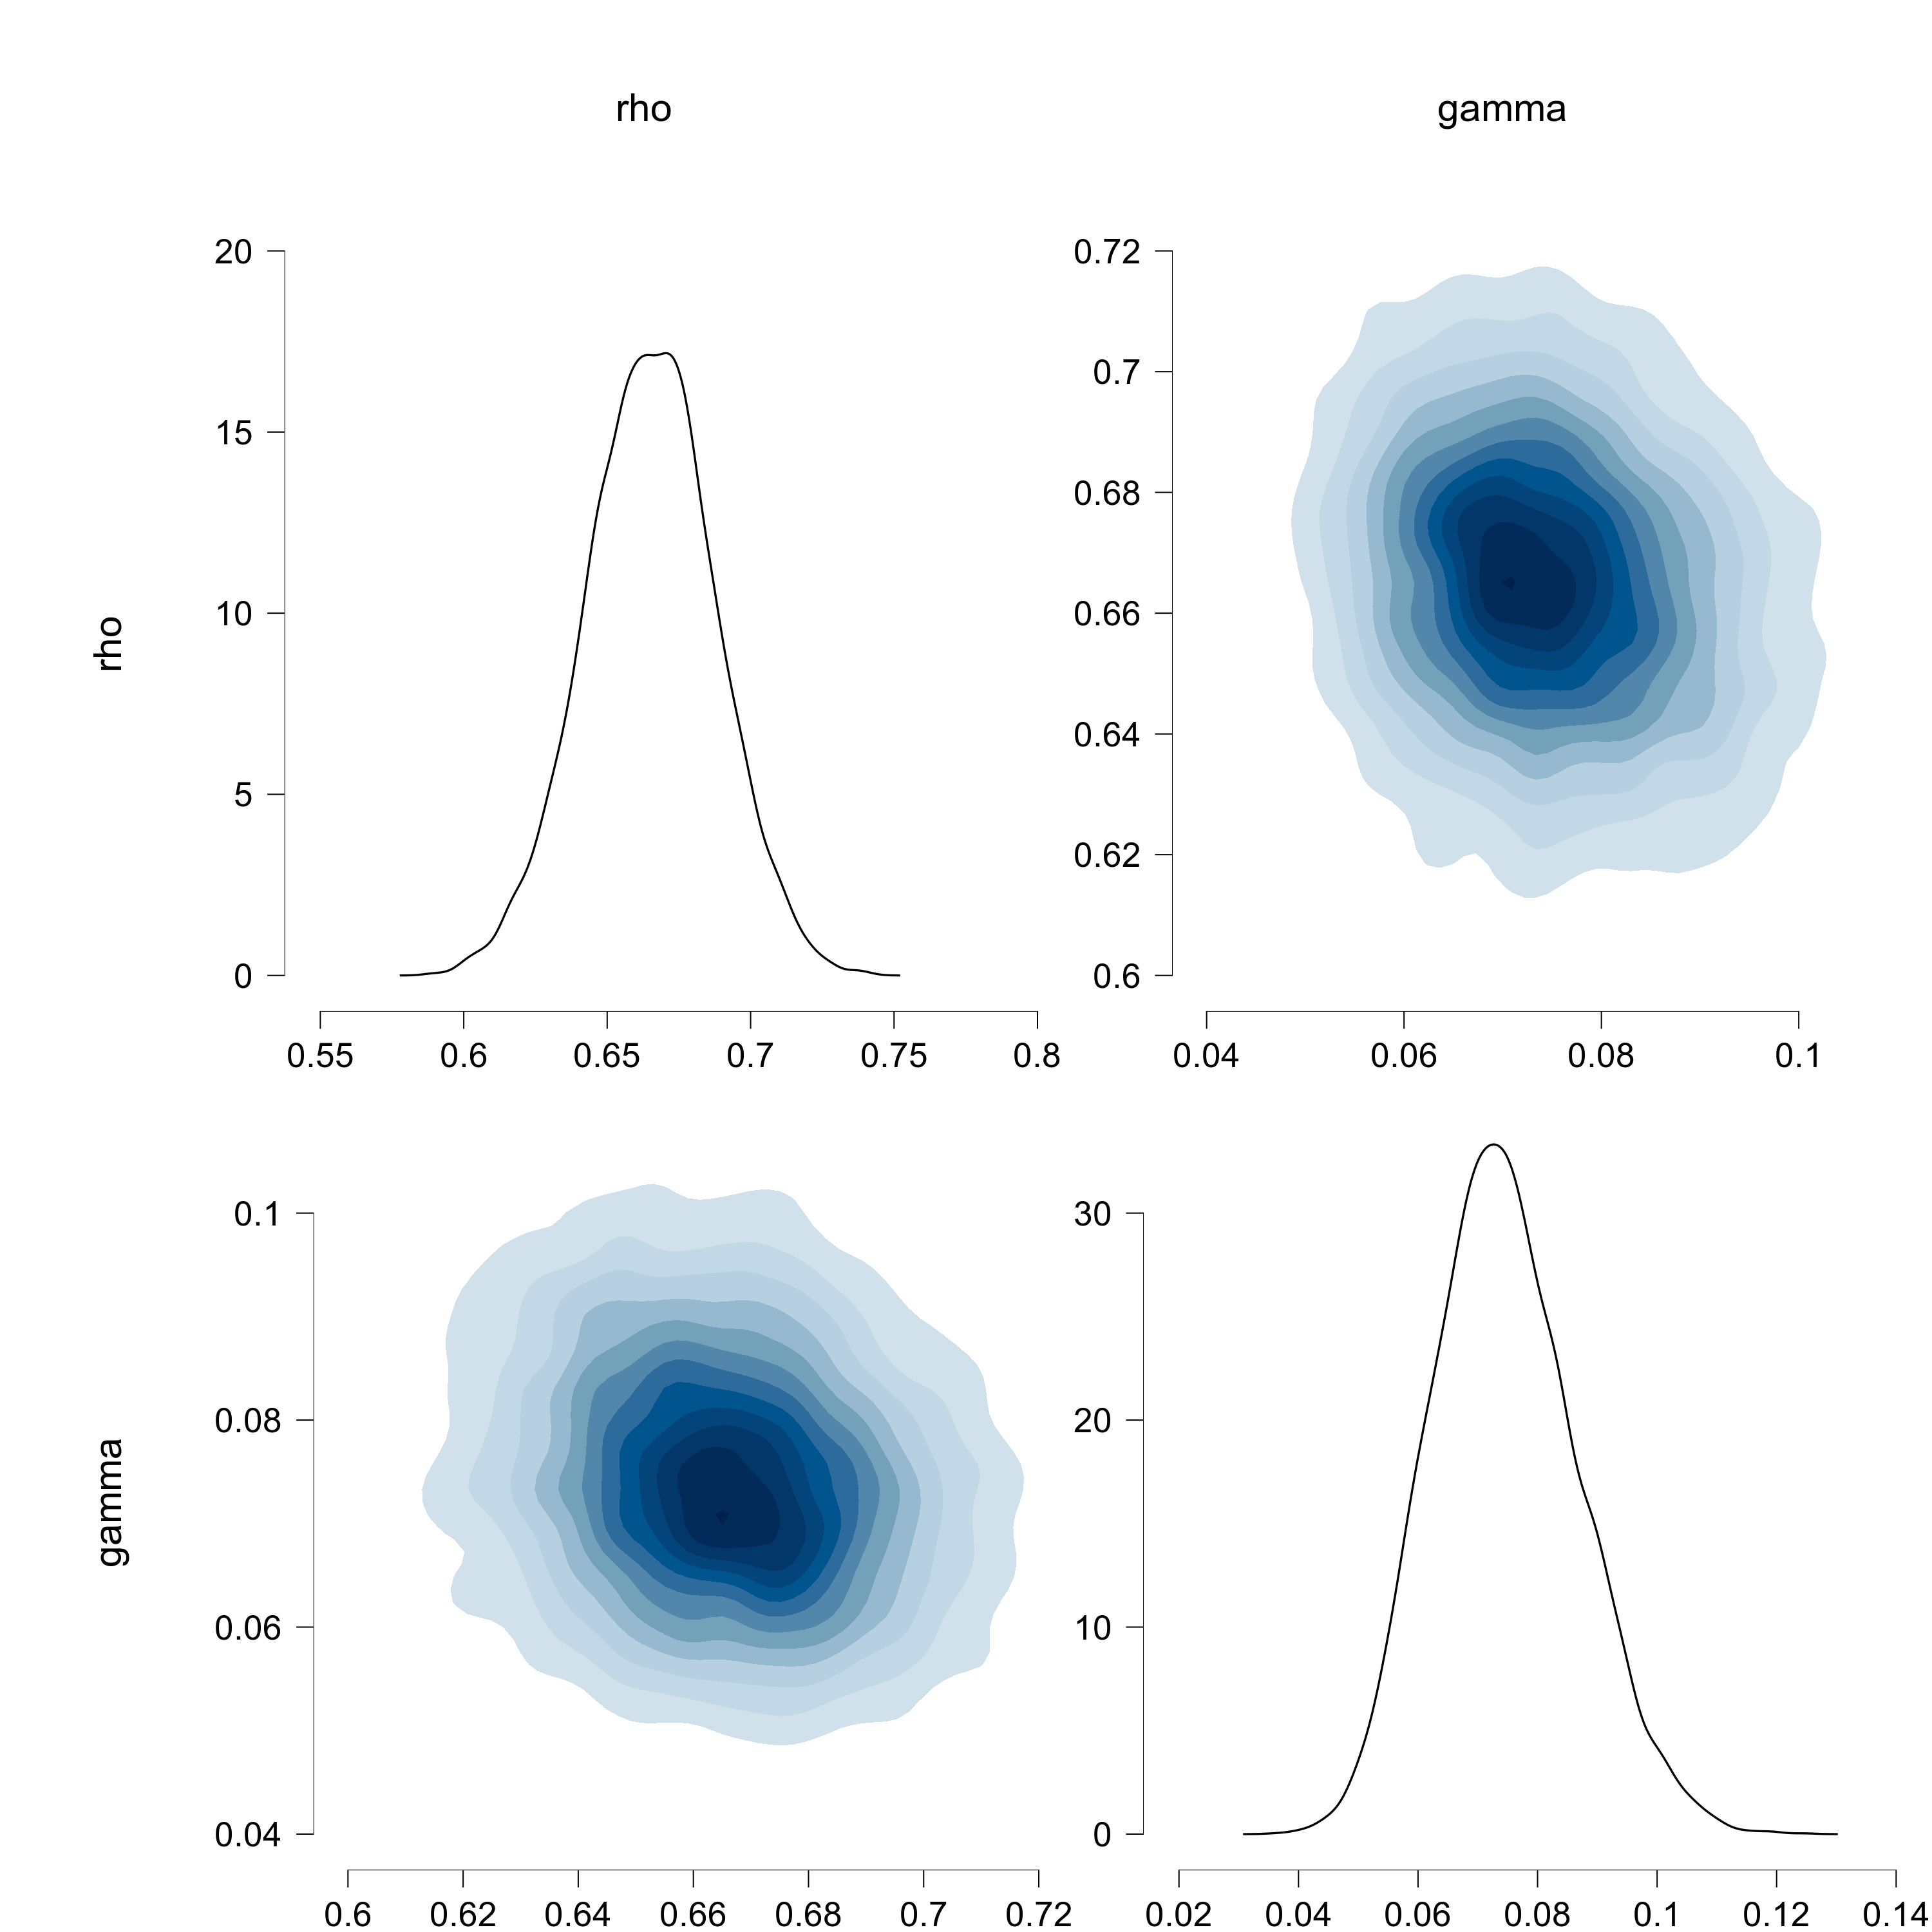
\includegraphics[width = 0.44\textwidth, trim = {3cm 0cm 15.02cm 19cm}, clip]{oneHighThreshold_1_betaAmyloidPositive_bivariate.eps}\pause
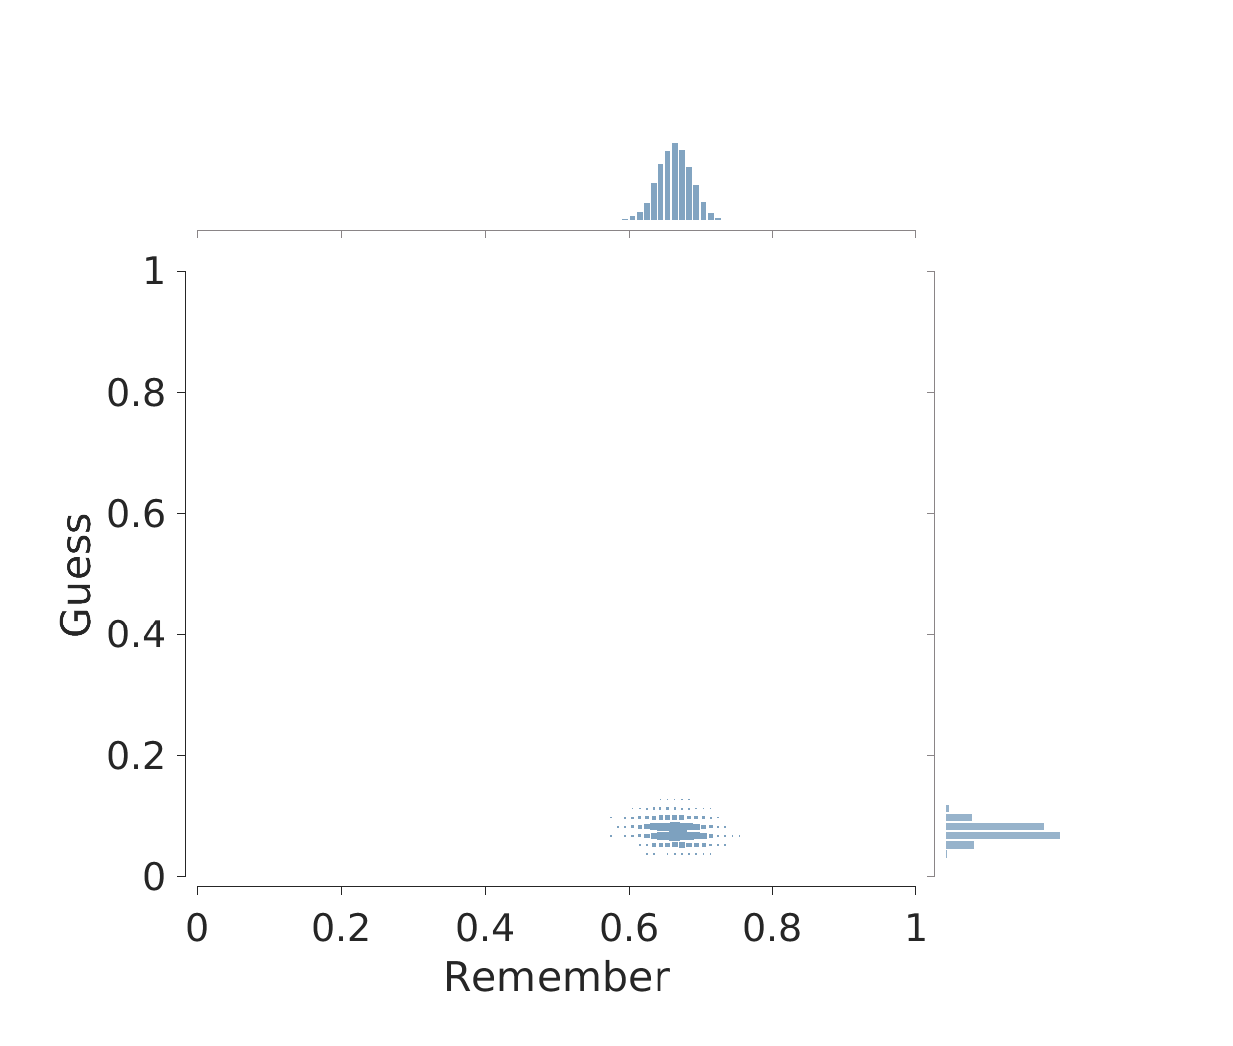
\includegraphics[width = 0.54\textwidth, trim = {0cm 1.8cm 3cm 2.25cm}, clip]{oneHighThreshold_1_betaAmyloidPositive.eps}
	\end{center}
\end{frame}




\end{document}
